\documentclass[deposito, acronym, symbols]{fei}

%\usepackage{glossaries}
\usepackage{subcaption} 
\usepackage{float}
%\usepackage{units}
\usepackage[portuguese]{algorithm2e}
\usepackage{biblatex}
\usepackage{amsmath}
\usepackage{listings}
\lstset{frame=tb,
language=Matlab,
aboveskip=3mm,
belowskip=3mm,
showstringspaces=false,
columns=flexible,
basicstyle={\small\ttfamily},
numbers=left,
numberstyle=\tiny\color{gray},
keywordstyle=\color{blue},
commentstyle=\color{dkgreen},
stringstyle=\color{mauve},
breaklines=true,
breakatwhitespace=true,
tabsize=4,
frame=shadowbox,
literate= {á}{{\'a}}1 {â}{{\^a}}1 {ã}{{\~a}}1 {é}{{\'e}}1 {ê}{\^e}1 {ç}{\c{c}}1 {í}{\i}1 {ú}{\'u}1 {ó}{{\'o}}1 {ô}{{\^o}}1 {õ}{{\~o}}1 {Á}{{\'A}}1 {É}{{\'E}}1, }
%%
\usepackage{color}
\definecolor{dkgreen}{rgb}{0,0.6,0}
\definecolor{mauve}{rgb}{0.58,0,0.82}
\usepackage[utf8]{inputenc}
\usepackage{chngcntr} %Faz com que o numero das notas de rodape aumente crescentemente.
\usepackage{appendix}
\counterwithout{footnote}{chapter}% "
\usepackage{siunitx}
\sisetup{output-exponent-marker=\ensuremath{\mathrm{e}}} %Escrita que precede cada entrada na lista de ilustrações.
\renewcommand{\cftfigurepresnum}{Figura }
\setlength{\cftfigurenumwidth}{5.7em}

\usepackage{titling}

%\makeglossaries
%%\newacronym[] {achpt} {ACT} {Aparecido ChupeTão}

\newacronym[longplural=Associações Brasileiras de Normas Técnicas]{abnt}{ABNT}{Associação Brasileira de Normas Técnicas}

\newacronym{ibge}{IBGE}{Instituto Brasileiro de Geografia e Estatística}

\newacronym{ashrae}{ASHRAE}{\textit{American Society of Heating, Refrigerating and Air-Conditioning Engineers}}

\newacronym{nbr}{NBR}{Norma Brasileira}

\newacronym{pmv}{PMV}{\textit{Predicted Mean Vote}}
	
\newacronym{ppd}{PPD}{\textit{Predicted Percentage of Dissatisfied}}
		
\newacronym{vgd}{VGD}{Ventilação Geral Diluidor}
		
\newacronym{vgl}{VGL}{Ventilação Local Exaustora}
		
\newacronym{cfd}{CFD}{\textit{Computational Fluid Dynamics}}
		
\newacronym{pcb}{PCB}{\textit{Printed Circuit Board}}
		
\newacronym{sms}{SMS}{\textit{Short Message Service}}
		
%\newglossaryentry{pi}{parent=greek,type=symbols,name={\ensuremath{\pi}},sort=p,description={número irracional que representa [razão entre a circunferência de qualquer círculo e seu diâmetro]}}
		


\title{Análises do sistema frontal da equipe RoboFEI SSL}
\author{ Felipe Estevão Coquito de Mello \\ Gabriel Mola da Silva \\ Netuno Trindade Torrente Rovaroto \\ Vitoria Fedatto Stefaneli}
\cidade{São Bernardo do Campo}
\instituicao{Centro Universitário FEI}

\addbibresource{Referencias.bib}
%\bibliographystyle{plain}
\bibliography{Referencias}
\graphicspath{ {Imagens/}, {Tabelas/}}

\begin{document}
\maketitle

\listoffigures

\chapter{Introdução e Objetivos}

\section{ROBOCUP}

A primeira proposição de que robôs poderiam jogar futebol veio do professor inglês Alan Mackworth no artigo “On Seeing Robots” em 1992. No mesmo ano em Tokyo, um grupo de pesquisadores japoneses realizaram um Workshop sobre os Grandes Desafios da Inteligências Artificiais, através de uma série de discussões proporão o uso do futebol para promover o desenvolvimento na área. Em junho de 1993, no Japão, foi fundada a competição de robótica “Robot J-League”, e no mesmo ano, a comunidade internacional pediu para a extensão internacional da competição, nascendo assim a “Robot World Cup Initiative” \cite{history}.

Para promover a robótica e a Inteligência Artificial a RoboCup traçou uma meta para sua competição, assim criando um marco caso seja concretizada. A meta consiste que em 2050 uma equipe composta apenas por robôs autônomos jogarem e ganharem contra o time vencedor da copa do mundo daquele ano, com base nas regras oficiais da FIFA \cite{objective}. Atualmente a RoboCup possui equipes tanto do ensino superior quanto do ensino básico que disputam diversas categorias, em eventos tanto de nível nacional quanto a nível internacional, como RoboCup Soccer, RoboCup Rescue, RoboCup@home e a RoboCup Juniora.

\subsection{Small Size League}

É uma das ligas mais antigas da RoboCup Soccer, tendo o foco em solucionar o problema da cooperação e controle de robôs inteligentes num ambiente altamente dinâmico com um sistema híbrido centralizado/distribuído \cite{about}. A partida ocorre entre duas equipes no 6 x 6 (Div. B) ou 11 x 11 (Div. A), onde um dos robôs de cada equipe é limitado a linha do gol, sendo este o único jogador permitido a tocar na bola dentro da área sem cometer uma penalidade. Os robôs são totalmente autônomos e omnidirecionais, entretanto a liga possui regulamento fixos em relação ao tamanho máximo dos jogadores na partida sendo necessário que todos sem exceção caibam em um cilindro de 180 mm de diâmetro e 150 mm altura, além de outras restrições da sua forma \cite{rules}.

\subsection{Conjunto Frontal}

O Frontal do robô é composto do “Roller System”, que atua como o controlador dinâmico do robô, sendo responsável pela condução da bola durante a partida. Atualmente a liga possui a regra que o robô pode cobrir no máximo 20\% da área total da bola, o que cria uma limitação estrutural para as equipes. Tendo isso em vista, o sistema frontal das equipes, geralmente é composto de um motor “Brushless”, um sistema de engrenagens ou correias e um cilindro de material polimérico (“Roller”). A equipe RoboFEI utiliza um motor Maxon EC-max-22 25W 18V, um engrenamento de 1:1:1 e um “Roller” de TPU Shore 30A. Nesse trabalho temos como objetivo analisar o conjunto frontal desenvolvido pela equipe e anilisar os esforços resultantes nas engrenagens do "Roller System".


\chapter{Fundamentação Téorica}

\section{Téoria}

\subsection{Tipos de Análises}
Antes de iniciarmos a nossa discussão acerca da fundamentação teórica, é necessário destacar a tamanha importância do software ANSYS utilizado durante o desenvolvimento deste projeto. Neste contexto, podemos definir o programa ANSYS, como sendo um software de elementos finitos que pode ser utilizado nas mais diversas classes de problemas de engenharia.

A incrível capacidade do ANSYS nos permite resolver diversos tipos de análises estruturais disponíveis, tais como: Análise estática (usada para deslocamentos e tensões); análise modal (calcula os modos de vibração de uma estrutura); análise harmônica (resposta de uma estrutura em cargas harmônicas variáveis no tempo); análise dinâmica transiente (resposta de uma estrutura à cargas arbitrariamente variáveis no tempo); análise espectral (assim como a analise modal, calcula tensões e deformações porém a partir de vibrações aleatórias); analise de flambagem (calcula as cargas de flambagem de uma estrutura); análise dinâmica explícita (calcula soluções rápidas para cargas dinâmicas). 

\subsection{Etapas do Processamento}

Para realizar a análise do nosso projeto, sendo elas: pré-processamento, cujo objetivo é realizar a modelagem da estrutura que se deseja analisar, a definição do tipo de elemento, as constantes características e o tipo do material, assim como a numeração dos nós e das barras; processamento, que consiste na simulação numérica, nela sendo Diante disso, torna-se notável a imensa importância do ANSYS para a solução de diversos problemas atuais da engenharia, assim como o problema abordado neste estudo. Dessa maneira, seguimos algumas etapas fundamentais realizada a definição das forças atuante da estrutura e suas condições de apoio, além da escolha do tipo de análise; pós-processamento, onde é feita a apresentação dos resultados do processamento, através de visualização gráfica e de resultados.

\subsection{Elementos Finitos}
Focalizando nosso estudo nos elementos finitos, define-se como uma técnica numérica amplamente usada na engenharia para resolver problemas complexos. O MEF envolve a subdivisão do domínio em pequenos elementos finitos e a aproximação da solução através de funções dentro de cada elemento. Essa abordagem permite a formulação de um sistema de equações que representa o problema físico, e a solução é obtida resolvendo-se numericamente esse sistema. O método dos elementos finitos é flexível, podendo ser aplicado a uma imensa gama de problemas em diversas áreas da engenharia, sendo uma ferramenta poderosa para análise e projeto de sistemas físicos. Vale ressaltar que, a malha pode ser refinada em certas áreas da estrutura, permitindo uma maior acurácia em regiões especificas.

\subsection{Convergência de Malha}
Ademais, iremos abordar brevemente o conceito de convergência de malha, que consiste na qualidade da malha, ou seja, qual seria o melhor tamanho de elemento para analisar cada caso, tendo uma boa qualidade de malha e não alterando consideravelmente o modelo numérico. Com isso em mente, será realizada a construção de um gráfico para viabilizarmos a evolução do refino de malha, indo de uma malha mais grosseira até uma mais elaborada, e quanto isso influenciará no ganho de precisão da análise, até um ponto que esse ganho seja irrelevante em função do número de elementos utilizados a cada caso.

\subsection{Análises Estruturais (Estático X Dinâmico)}

Estática: efeitos inerciais desprezados e o tempo de duração não muda os resultados
Dinâmica: efeitos inerciais importantes e o tempo de duração influencia os resultados
A partir desses conceitos, iremos pautar nosso estudo na dinâmica, pois queremos analisar o comportamento do engrenamento do sistema “Roller” ao longo do tempo, não desconsiderando os efeitos inerciais

\section{Desenho}

O modelo das engrenagens foi desenvolvido pela equipe RoboFEI e pode ser extraída a partir do seu repositório online \cite{git}, iremos focar nosso estudo nas 3 engrenagens que faz parte do sistema de transmissão. Para o estudo usaremos apenas as duas primeiras engrenagens da transmissão.

Engrenagem Motriz: Z1 = 18 dentes ; d1 = 9 mm ; m1 = 0,5

Engrenagem Intermediaria:  Z2 = 18 dentes ; d2 = 9 mm ; m2 = 0,5

\begin{figure}[!htb]
 \centering
    \caption{Engrengagens Estudadas}
    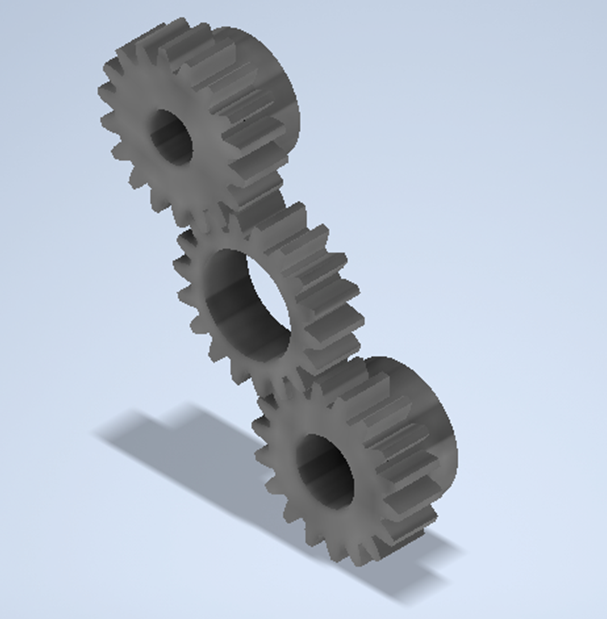
\includegraphics[width=0.5\linewidth]{Imagens/Engrenagens.png}
    \smallcaption{Fonte: Autor}
    \label{fig: Estrutura do Projeto}
 \end{figure}

\chapter{Ansys}
Nesta seção, descreveremos os parâmetros relevantes a serem considerados durante a nossa análise, a malha utilizada e o setup do projeto. A seguir, ampliaremos o texto e faremos as correções necessárias.

\section{Malha}
Dando sequência, é importante definir a malha utilizada cuidadosamente para realizar as simulações e análises, visto que devemos realizar uma convergência de malha, chegando em um número de elementos suficientemente bom para representar nosso modelo, mas não sendo excessivo (evitando trabalho computacional desnecessário). Nossa malha escolhida tem 366217 elementos e 527878 nós, considerando critério de 3%.

\begin{figure}[!htb]
 \centering
    \caption{Malha das Engrengagens Estudadas}
    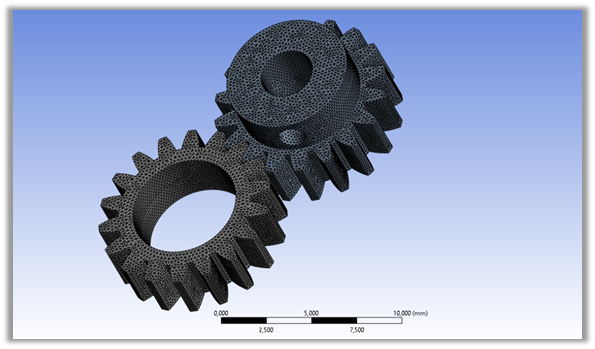
\includegraphics[width=0.9\linewidth]{Imagens/malha.png}
    \smallcaption{Fonte: Autor}
    \label{fig: Convergência de Malha}
 \end{figure}

\begin{figure}
 \centering
    \caption{Convergência de Malha Deformação}
    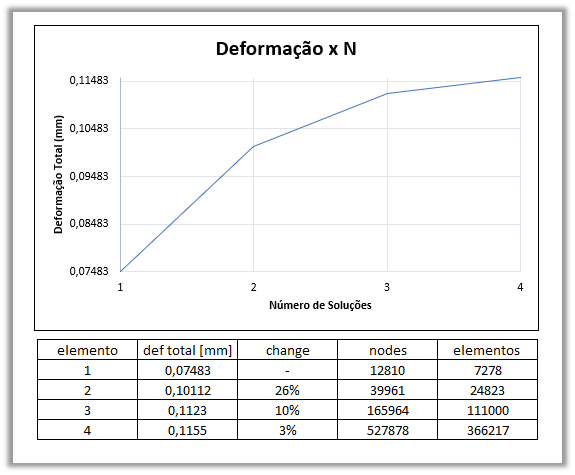
\includegraphics[width=0.8\linewidth]{Imagens/Deformação x N.png}
    \smallcaption{Fonte: Autor}
    \label{fig: Deformação x N}
 \end{figure}

\begin{figure}
 \centering
    \caption{Convergência de Malha Tensão}
    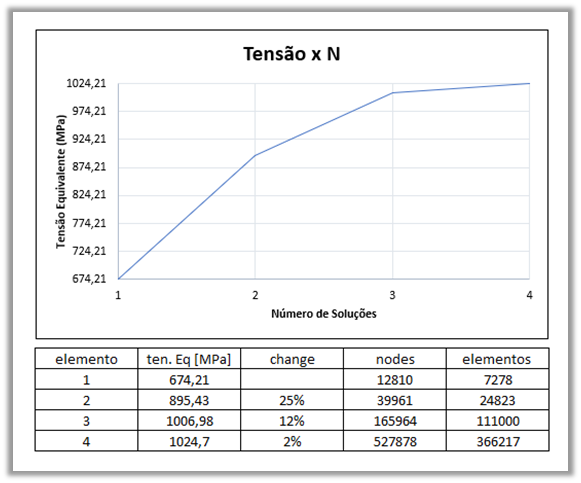
\includegraphics[width=0.8\linewidth]{Imagens/Tensão x N.png}
    \smallcaption{Fonte: Autor}
    \label{fig: Tensão x N}
 \end{figure}
 
 \newpage
 
\section{Setup}
Iniciando nossa introdução ao setup, estão disponíveis as 3 análises desenvolvidas no trabalho, sendo elas: análise estática estrutural, dinâmica e modal.

\begin{figure}[!htb]
 \centering
    \caption{Setup Geral}
    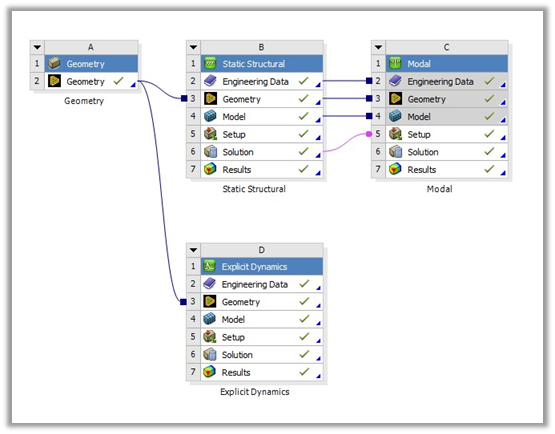
\includegraphics[width=0.8\linewidth]{Imagens/setup1.png}
    \smallcaption{Fonte: Autor}
    \label{fig: Setup do Workbench}
 \end{figure}
 
 \begin{figure}[!htb]
 \centering
    \caption{Setup da Análise Dinâmica}
    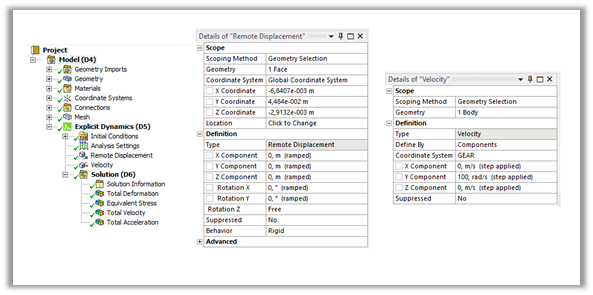
\includegraphics[width=0.8\linewidth]{Imagens/setup dinamico.png}
    \smallcaption{Fonte: Autor}
    \label{fig: Setup do Workbench}
 \end{figure}
 
 \begin{figure}[!htb]
 \centering
    \caption{Setup da Análise Estática}
    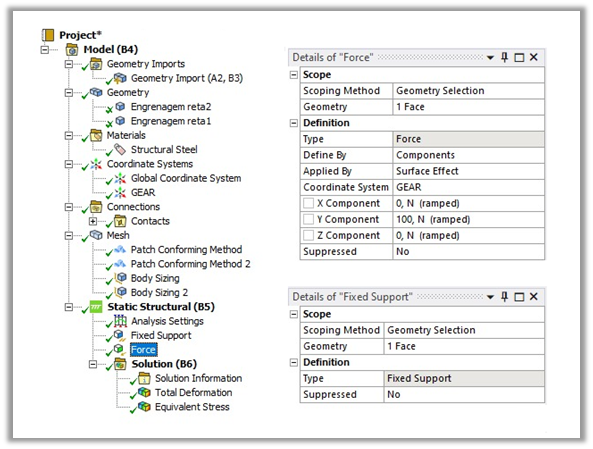
\includegraphics[width=0.8\linewidth]{Imagens/setup estrutural.png}
    \smallcaption{Fonte: Autor}
    \label{fig: Setup do Workbench}
 \end{figure}
 
\begin{figure}[!htb]
 \centering
    \caption{Setup do Modal}
    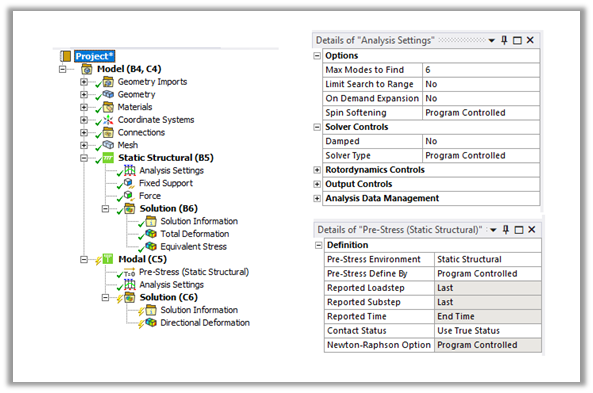
\includegraphics[width=0.8\linewidth]{Imagens/modal.png}
    \smallcaption{Fonte: Autor}
    \label{fig: Setup do Workbench}
 \end{figure}
 
 \newpage
 
\section{Solution}
Abaixo serão apresentadas as escolhas de soluções feitas pelo grupo que melhor forneciam os resultados mais relevantes para a situação proposta.

 \begin{figure}[!htb]
 \centering
    \caption{Solução Dinâmica}
    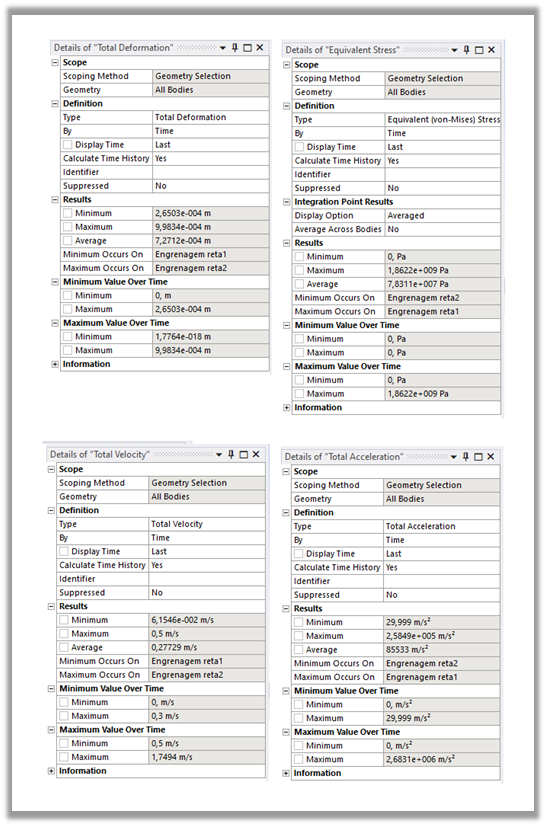
\includegraphics[width=0.95\linewidth]{Imagens/solução dinamica.png}
    \smallcaption{Fonte: Autor}
    \label{fig: Setup do Workbench}
 \end{figure}
 
\begin{figure}[!htb]
 \centering
    \caption{Setup Estática}
    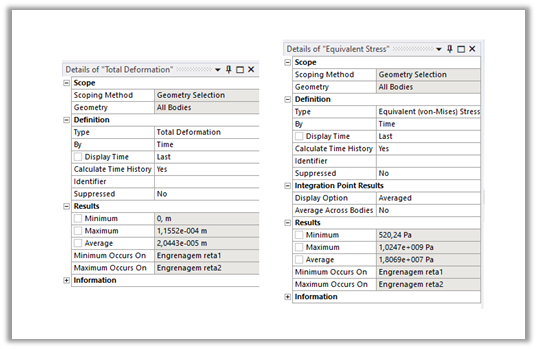
\includegraphics[width=1\linewidth]{Imagens/solução estatica.png}
    \smallcaption{Fonte: Autor}
    \label{fig: Setup do Workbench}
 \end{figure}
\begin{figure}[!htb]
  
 \centering
    \caption{Solução do Modal}
    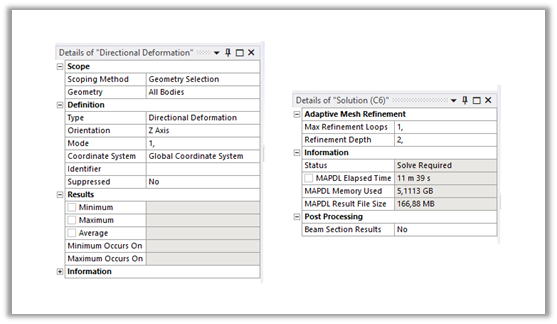
\includegraphics[width=1\linewidth]{Imagens/solução modal.png}
    \smallcaption{Fonte: Autor}
    \label{fig: Setup do Workbench}
 \end{figure}
 
\chapter{Resultado e Discussão}
 Agora serão apresentados e brevemente comentados e discutidos os resultados obtidos ao longo de nosso estudo e através dos 3 modos de analise utilizados: 
 \section{Resultados da analise estática}
 
\begin{figure}[!htb]
 \centering
    \caption{Deformação Total}
    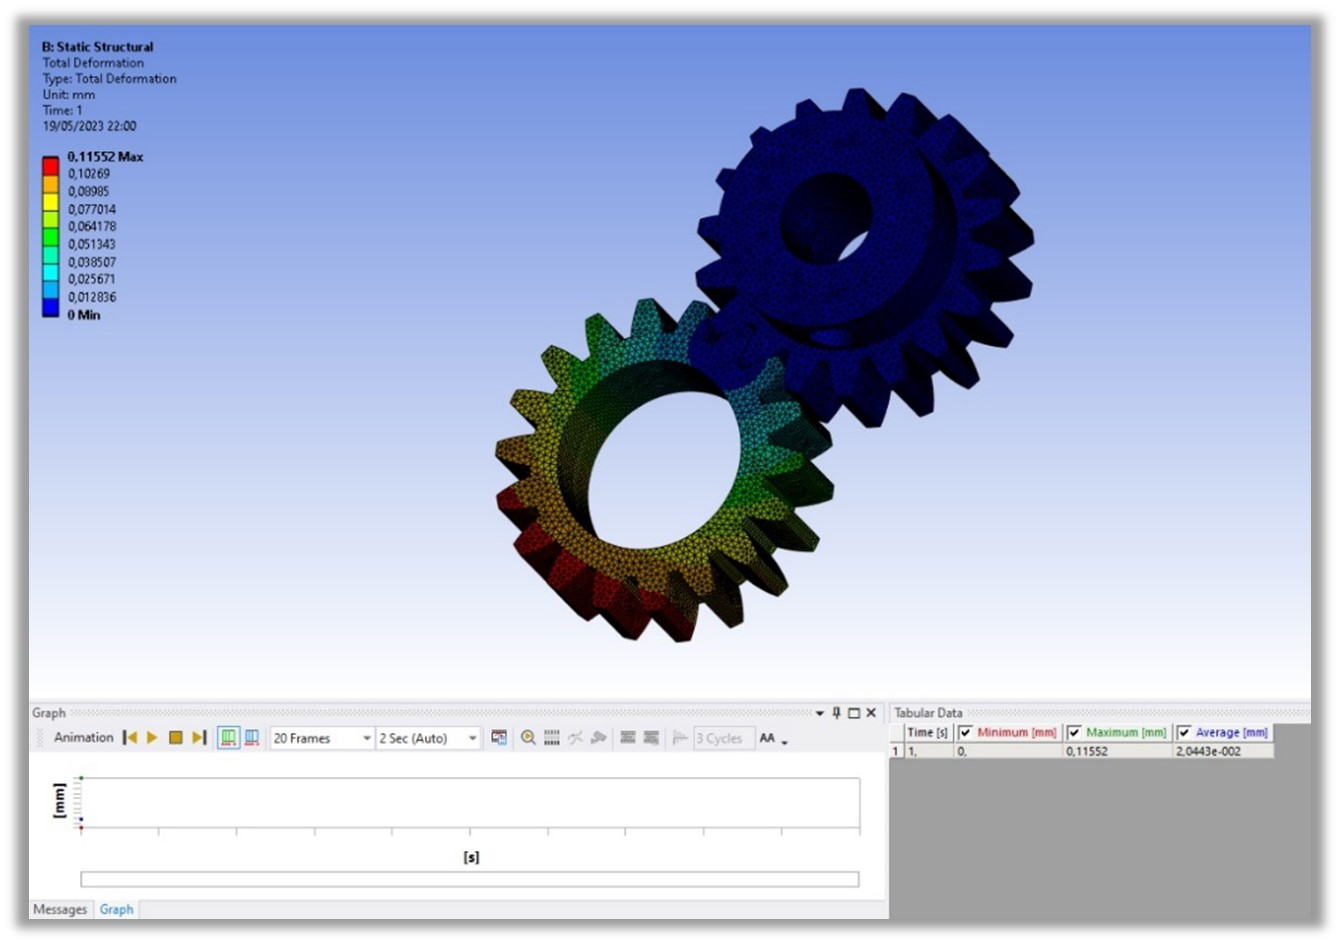
\includegraphics[width=1\linewidth]{Imagens/def total estatico.jpg}
    \smallcaption{Fonte: Autor}
    \label{fig: Setup do Workbench}
 \end{figure}
 
 Através dos parâmetros e soluções apresentados anteriormente, chegamos a conclusão de que a deformação total máxima é de 0,11552 mm, o que corresponde a valores aceitaveis e esperados no nosso projeto. 
 
\begin{figure}[]
 \centering
    \caption{Tensão Equivalente}
    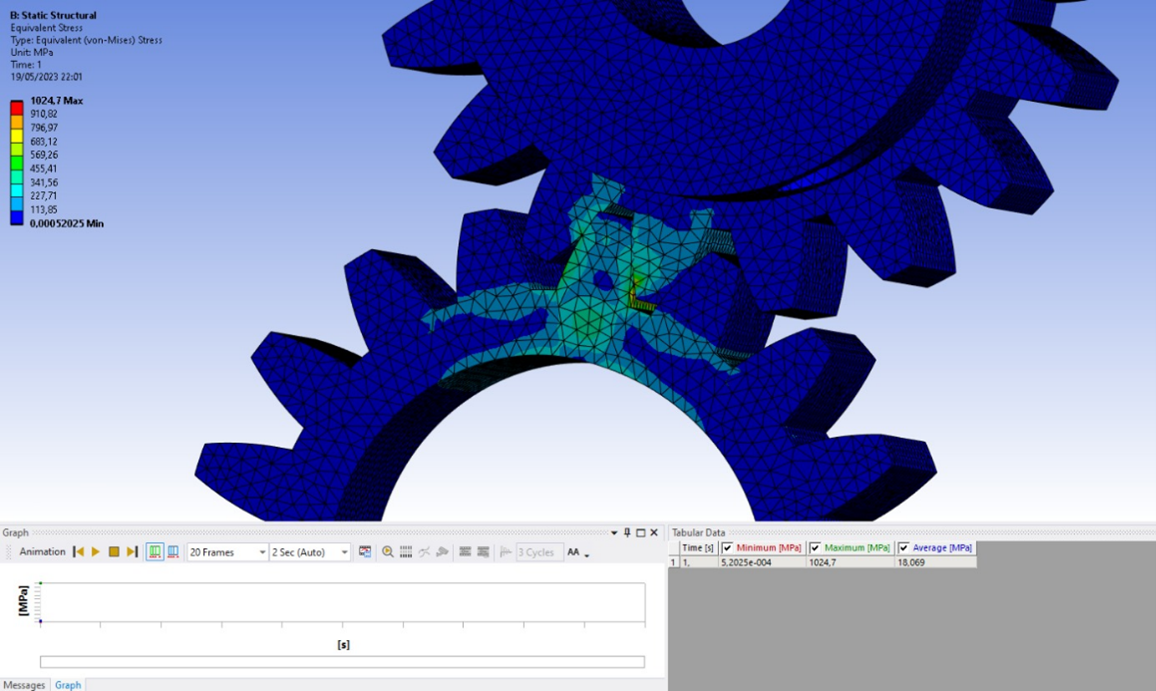
\includegraphics[width=1\linewidth]{Imagens/ten eq estatico.png}
    \smallcaption{Fonte: Autor}
    \label{fig: Setup do Workbench}
 \end{figure}
 
\begin{figure}[]
 \centering
    \caption{Deformação Total dos dentes da engrenagem motora}
    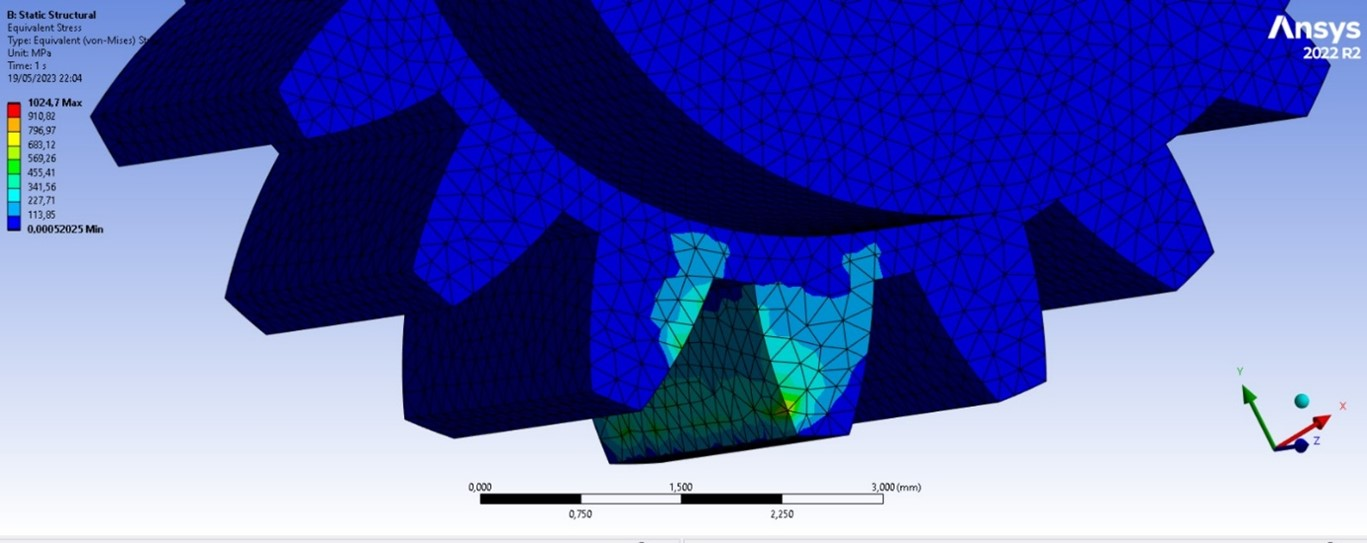
\includegraphics[width=1\linewidth]{Imagens/def total cima.jpg}
    \smallcaption{Fonte: Autor}
    \label{fig: Setup do Workbench}
 \end{figure}
 
\begin{figure}[]
 \centering
    \caption{Deformação Total dos dentes da engrenagem movida}
    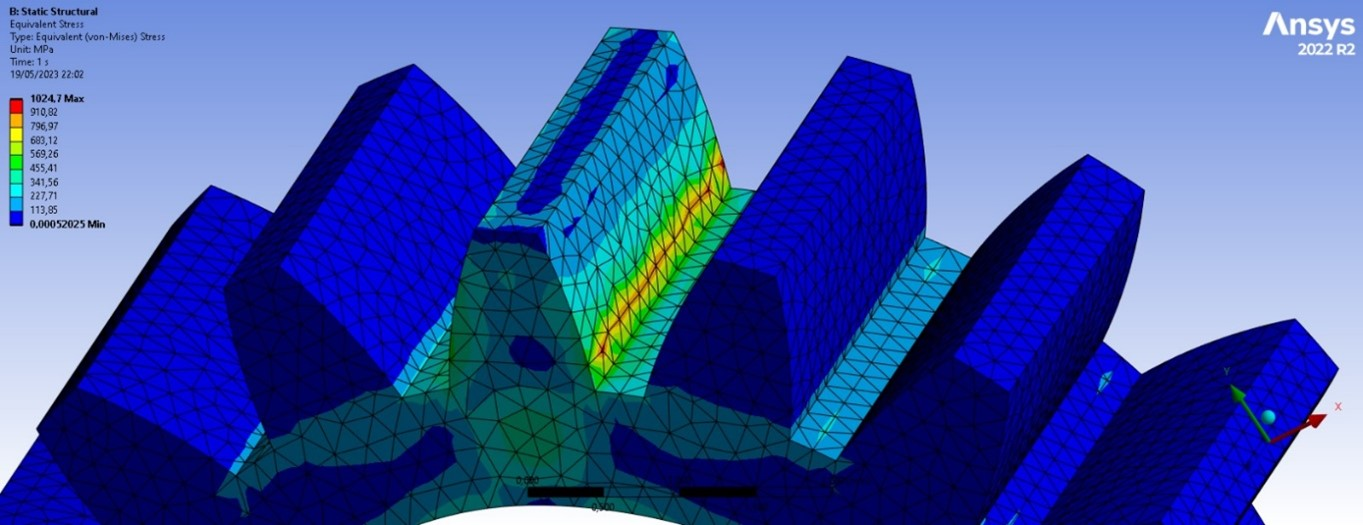
\includegraphics[width=1\linewidth]{Imagens/def total baixo.jpg}
    \smallcaption{Fonte: Autor}
    \label{fig: Setup do Workbench}
 \end{figure}
 
\newpage

\section{Resultados da analise dinâmica}



\begin{figure}[]
 \centering
    \caption{Deformação Total}
    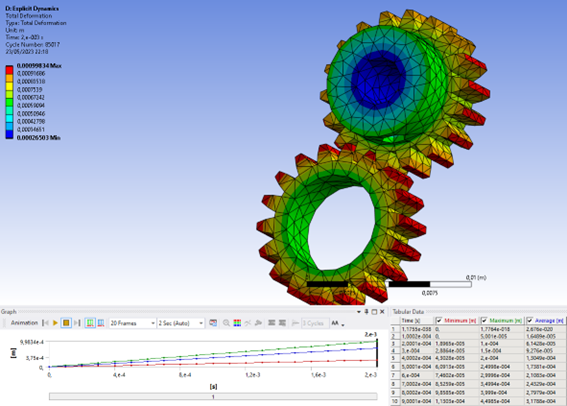
\includegraphics[width=1\linewidth]{Imagens/def total dinamica.png}
    \smallcaption{Fonte: Autor}
    \label{fig: Setup do Workbench}
 \end{figure}
 
\begin{figure}[]
 \centering
    \caption{Tensão Equivalente}
    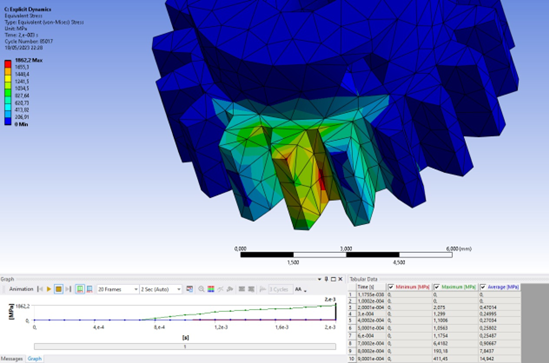
\includegraphics[width=1\linewidth]{Imagens/ten eq dinamica.png}
    \smallcaption{Fonte: Autor}
    \label{fig: Setup do Workbench}
 \end{figure}
 
\begin{figure}[]
 \centering
    \caption{Relação da deformação total com a velocidade}
    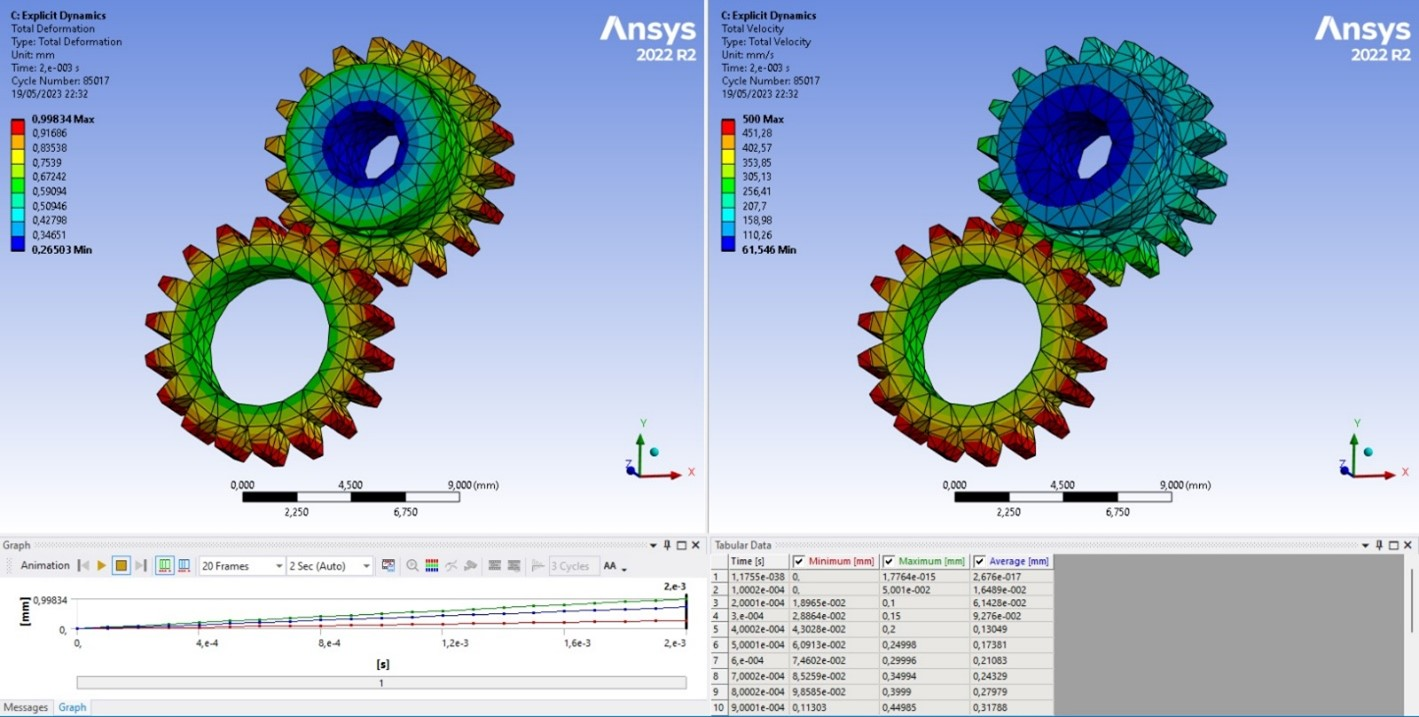
\includegraphics[width=1\linewidth]{Imagens/def eq x vel total.jpg}
    \smallcaption{Fonte: Autor}
    \label{fig: Setup do Workbench}
 \end{figure}
 
\newpage
 
\section{Resultados da analise modal}

Nesta análise é possível ver a forma de vibrar do sistema em todas os eixos do modelo, através da análise Modal. Através dessa análise é possível ver as Deformações Direcionais em cada frequência do modelo. A frequência mais comum de ocorrer a ressonância seria a no Eixo Y, a que sofre esforço do sistema.

 \begin{figure}[!htb]
  \centering
    \caption{Modos de Vibrar no Eixo X}
    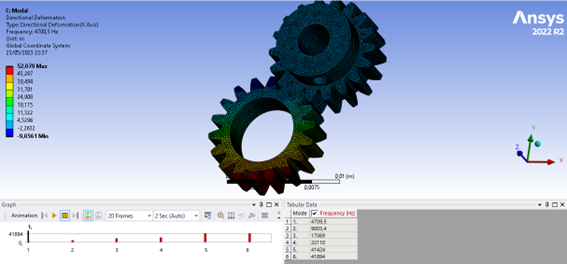
\includegraphics[width=1\linewidth]{Imagens/modal x.png}
    \smallcaption{Fonte: Autor}
    \label{fig: Setup do Workbench}
 \end{figure}
 
 \begin{figure}[!htb]
   \centering
    \caption{Modos de Vibrar no Eixo Y}
    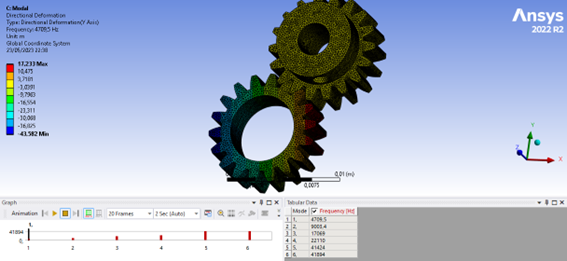
\includegraphics[width=1\linewidth]{Imagens/modal y.png}
    \smallcaption{Fonte: Autor}
    \label{fig: Setup do Workbench}
 \end{figure}
 
 \begin{figure}[!htb]
  \centering
    \caption{Modos de Vibrar no Eixo Z}
    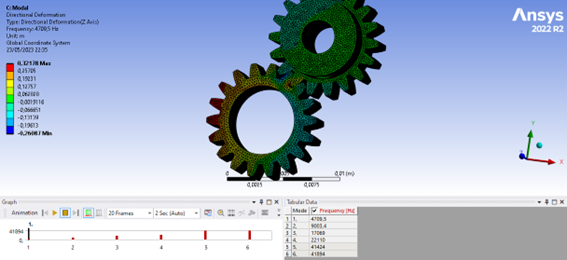
\includegraphics[width=1\linewidth]{Imagens/modal z.png}
    \smallcaption{Fonte: Autor}
    \label{fig: Setup do Workbench}
 \end{figure}
 
\chapter{Conclusão}

Diante dos dados supra apresentados, torna-se notável a grande importância da utilização do ANSYS em projetos, a fim de retirar informações valiosas a partir do método dos elementos finitos e da análise de estruturas. Em uma situação real essa análise poderia levar a uma melhor compreensão do problema estudado, otimizando dessa maneira os processos produtivos e construtivos. Ademais, é importante ressaltar que com o aprofundamento do uso do software ANSYS e com os ensinamentos adquiridos durante o semestre, se tornou possível realizar esta análise completa obtendo os resultados desejados, e concluir que eles são fidedignos aos resultados esperados para esse componente do RoboFEI.

\printbibliography[type=online]
\nocite{*}

\end{document}